\documentclass{ximera}

%\addPrintStyle{..}

\begin{document}
	\author{Bart Lambregs}
	\xmtitle{De mathematische slinger}{}
    \xmsource\xmuitleg





	%%%\section{De mathematische slinger}

	Als tweede voorbeeld bekijken we een massa aan een touw. Geen erg spectaculair systeem, zal je denken. Toch zal je snel zien dat de beweging verre van eenvoudig is.
	
	Stel dat we te maken hebben met een slinger van lengte $l$ die bovenaan bevestigd is en waaraan een massa $m$ hangt. De wrijving laten we buiten beschouwing. We beschouwen ook een model waarin het touw geen massa heeft.\footnote{Moesten we dit wel in rekening brengen, dan zouden we het model de fysische slinger noemen.} De positie van de slinger kunnen we aangeven d.m.v. de booglengte, gemeten vanaf de evenwichtspositie tot aan de massa. De hoek die het touw met de verticale maakt, is een mogelijk alternatief. 
	
	Om de beweging te kunnen vinden d.m.v. de tweede wet van Newton, maken we een krachtendiagram. We voeren een assenstelsel rakend aan de baan van het voorwerp in. De richting rakend aan de baan noemen de tangentiële richting, die loodrecht op de baan noemen we de normale richting. Natuurlijk kunnen we ook altijd voor een $x$-as en een $y$-as opteren.
	%%%\newline
	\begin{image}
	% \begin{wrapfigure}[11]{r}{0.33\textwidth}
	%
	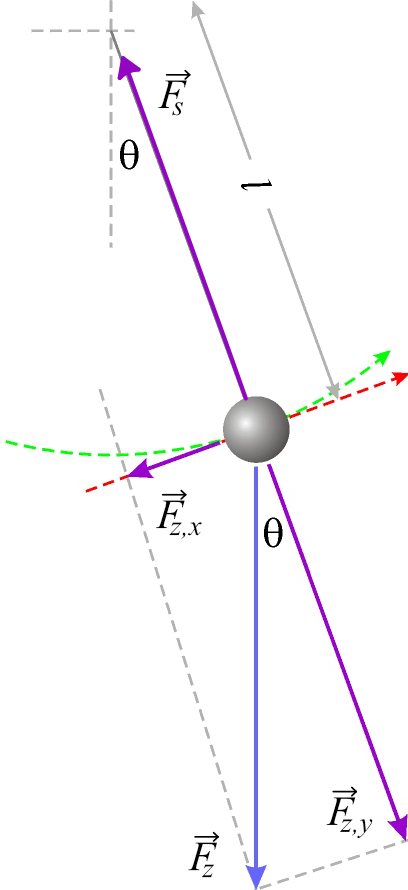
\includegraphics[width=0.34\textwidth]{pendulum}
	%\captionof{figure}{A gull}
	% \end{wrapfigure}
	\end{image}
	Volgens de normale richting zal de spankracht in het touw in combinatie met de normale component van de zwaartekracht voor de nodige middelpuntzoekende kracht zorgen. De massa beweegt immers op een cirkel met variërende snelheid waardoor ook een variërende middelpuntzoekende kracht nodig is. Echter kunnen we volgens deze richting niet veel leren over de manier waarop de massa heen en weer slingert. Daarvoor hoeven we enkel de tangentiële richting te bekijken. We passen dan ook de tweede wet van Newton volgens deze richting toe. 
	\begin{gather*}
	F=ma\\
	\Downarrow\\
	-mg\sin\theta=m\frac{d^2s}{dt^2}\\
	\phantom{\theta=\frac{s}{l}}\Updownarrow\theta=\frac{s}{l}\\
	\frac{d^2s}{dt^2}+g\sin\left(\frac{s}{l}\right)=0
	\end{gather*}
	Dit is een \emph{niet}-lineaire differentiaalvergelijking. Ze is verre van eenvoudig om exact op te lossen. We hebben daartoe een veel zwaarder arsenaal aan wiskundige functies nodig dan dat wij op dit moment kennen. In feite is dat ook niet zo verwonderlijk. Wanneer we bijvoorbeeld de slinger vanuit een initiële hoek van 120 graden met een voldoende hoge beginsnelheid laten vertrekken, zal de slinger niet slingeren maar pulserende rondjes blijven draaien. Deze oplossing samen met bijvoorbeeld stil blijven hangen op 180 graden en nog andere varianten, zijn allemaal mogelijkheden die aan de differentiaalvergelijking moeten voldoen. Ingewikkeld dus.
	
	Wij zullen ons hier beperken tot kleine hoeken\footnote{Ik weet het, dat doet pijn aan het wiskundig exacte deel van ons hart, maar in feite is het in de fysica nooit anders \ldots \'Alles wat we in de fysica doen is een benadering van de realiteit. Zo hebben we bij onze slinger reeds de massa van het touw overboord gegooid, de massa van het object geen dimensie gegeven, gedaan alsof de wrijvingskracht niet bestaat, de zwaartekracht benaderd door $mg$ terwijl die eigenlijk afhankelijk is van de hoogte boven het aardoppervlak, de wetten van Newton gebruikt waar we eigenlijk de wetten van de kwantummechanica zouden moeten bovenhalen, gedaan alsof slingers het enige in het universum zijn \ldots }. In dat geval kunnen we de sinus van een argument benaderen door het argument zelf, $\sin\alpha\approx\alpha$. \footnote{Herinner je misschien dat je ooit de limiet $\displaystyle\lim_{x\rightarrow0}\frac{\sin x}{x}=1$ bewezen hebt.} \footnote{In feite is de wet van Hooke enzelfde lineaire benadering van de veerkracht. Die is ook maar geldig voor zolang we de veer niet te ver uitrekken. Willen we accurater zijn, dan moeten we termen afhankelijk van bijvoorbeeld $x^2$ in rekening brengen \ldots}
	\begin{image}
	
	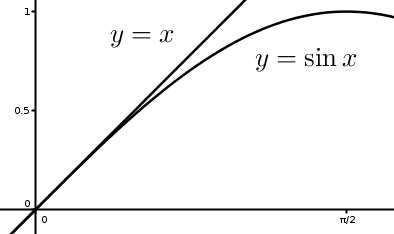
\includegraphics[width=0.4\textwidth]{sinx_x}
	\end{image}
	% \begin{minipage}[t]{.5\textwidth}
	% \begin{eqnarray*}
	% \sin\alpha\approx\alpha
	% \end{eqnarray*}
	% \end{minipage}
	% \begin{minipage}[t]{.4\textwidth}
	% \phantom{}
	% 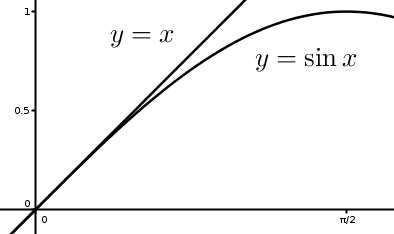
\includegraphics[width=\textwidth]{sinx_x}
	% \end{minipage}
	
	De differentiaalvergelijking wordt er dan een heel pak gemakkelijker op:
	\begin{eqnarray*}
	\frac{d^2s}{dt^2}+g\sin\left(\frac{s}{l}\right)&=&0\\
	&\rotatebox[origin=c]{-90}{$\rightsquigarrow$}&\mathrm{benadering} \sin\alpha\approx\alpha\\
	\frac{d^2s}{dt^2}+\frac{g}{l}s&=&0
	\end{eqnarray*}
	We vinden zo niets anders dan de differentiaalvergelijking van de harmonische trilling (\ref{diffvgl_ht}). De oplossing is wiskundig gezien dan ook dezelfde\footnote{Zo zie je maar hoe we een eenheid in verschillende verschijnselen kunnen terugvinden.}.
	\begin{gather*}
	\frac{d^2s}{dt^2}+\frac{g}{l}s=0\quad\Leftrightarrow\\
	%\Updownarrow\\
	s(t)=A\sin(\omega t+\varphi)\quad\mathrm{met}\quad\omega=\sqrt{\frac{g}{l}}
	\end{gather*}
	Realiseer je dat de amplitude hier de booglengte bij maximale uitwijking is. Ook zien we dat de slingerlengte de periode van de trilling bepaalt en dat de amplitude noch de massa hierop een invloed heeft \ldots
	\begin{eqnarray*}
	T=2\pi\sqrt{\frac{l}{g}},\quad f=\frac{1}{2\pi}\sqrt{\frac{g}{l}}
	\end{eqnarray*}
	
	%%\newpage
	
	


\end{document}
